\documentclass[11pt,a4paper]{article}
\usepackage[utf8]{vietnam}
\usepackage{mathptmx}
\usepackage[a4paper,top=1.8cm,bottom=1.9cm,left=2.2cm,right=2cm]{geometry}
\usepackage{graphicx}
\usepackage{booktabs}
\usepackage{tabularx}
\usepackage{array}
\usepackage{enumitem}
\usepackage{xcolor}
\usepackage{titlesec}
\usepackage{fancyhdr}
\usepackage{caption}
\usepackage[unicode,colorlinks=true,urlcolor=blue!60!black,linkcolor=black]{hyperref}

\definecolor{hust}{RGB}{176,0,32}
\titleformat{\section}{\large\bfseries}{\thesection.}{0.5em}{}
\titlespacing*{\section}{0pt}{9pt}{4pt}
\setlist{nosep,leftmargin=1.3em}
\setlength{\parindent}{0pt}
\setlength{\parskip}{3pt}
\captionsetup{font=small,labelfont=bf,skip=3pt}
\renewcommand{\arraystretch}{1.12}

\pagestyle{fancy}
\fancyhf{}
\renewcommand{\headrulewidth}{0pt}
\fancyfoot[L]{\small Nhóm 09 -- Báo cáo tiến độ bài tập lớn IT3190}
\fancyfoot[R]{\small Trang \thepage/3}

\begin{document}

% ------------------------------------------------------------------ tiêu đề
\begin{minipage}[c]{0.11\textwidth}
  
\includegraphics[height=2.15cm]{logo_hust.png}
\end{minipage}\hfill
\begin{minipage}[c]{0.86\textwidth}
  {\bfseries ĐẠI HỌC BÁCH KHOA HÀ NỘI}\\
  {\bfseries TRƯỜNG CÔNG NGHỆ THÔNG TIN VÀ TRUYỀN THÔNG}\\[2pt]
  IT3190 -- Nhập môn Học máy và Khai phá dữ liệu, học kỳ 2026.1\\[4pt]
  {\color{hust}\rule{\linewidth}{0.8pt}}
\end{minipage}

\vspace{6pt}
\begin{center}
  {\bfseries BÁO CÁO TIẾN ĐỘ BÀI TẬP LỚN -- NHÓM 09}\\[3pt]
  {\large\bfseries ƯỚC LƯỢNG GIÁ THUÊ PHÒNG TRỌ TẠI HÀ NỘI\\ TỪ DỮ LIỆU TIN ĐĂNG TRỰC TUYẾN}\\[6pt]
  \small
  \begin{tabular}{@{}l@{\hspace{2.2em}}l@{\hspace{2.2em}}l@{}}
    Phạm Thành Trung -- 20235853 & Lê Tuấn Trung -- 20235852 & Nguyễn Khánh Toàn -- 20235847\\
    Trần Việt Gia Khánh -- 20235756 & Hà Trọng Thắng -- 20235827 & \\
  \end{tabular}\\[4pt]
  Giảng viên hướng dẫn: TS. Nguyễn Kiêm Hiếu\\[2pt]
  Mã nguồn: \url{https://github.com/ToanKhanh137/DinhGiaPhongTro}
\end{center}
\vspace{-6pt}

% ------------------------------------------------------------------ 1
\section{Mô tả bài toán}
Sinh viên thuê trọ ở Hà Nội khó biết một tin đăng có giá hợp lý hay không. Nhóm xây dựng hệ thống học máy
\textbf{ước lượng giá thuê hợp lý (triệu đồng/tháng)} cho một phòng trọ từ thông tin trong tin đăng, kèm
\textbf{khoảng giá 80\%} của các phòng tương tự, để nhận xét giá chủ trọ đưa ra là đắt, hợp lý hay rẻ.
\begin{itemize}
  \item \textbf{Đầu vào:} diện tích, quận/phường, tình trạng nội thất, mô tả tin đăng (hoặc link tin đăng).
        \textbf{Đầu ra:} giá ước tính, khoảng giá 80\%, nhận xét so với giá chủ trọ.
  \item \textbf{Bài toán chính -- hồi quy} trên log(giá); đánh giá bằng MAE, MAPE, $R^2$ với
        cross-validation chia theo phòng (GroupKFold) để tránh rò rỉ do tin đăng lại.
  \item \textbf{Bài toán phụ:} phân loại loại tin (phòng riêng / ở ghép / nhiều mức giá) để lọc nhiễu nhãn;
        phân cụm khu vực trọ; khai phá luật kết hợp giữa tiện ích và mức giá; giao diện web dự đoán giá.
\end{itemize}

% ------------------------------------------------------------------ 2
\section{Các tập dữ liệu}
Dữ liệu do nhóm tự thu thập từ 3 trang rao vặt, khu vực Hà Nội, qua 7 lượt crawl từ 08/10 đến 15/11/2026.
Crawler tuân theo robots.txt, giãn cách 1,5 giây/request, không lưu tên hay tài khoản người đăng, che số điện thoại
trong mô tả; dữ liệu chỉ dùng cho học tập và không công bố lại.

\begin{table}[h]
\centering\small
\caption{Nguồn dữ liệu (số tin sau khi bỏ trùng theo mã tin)}
\begin{tabular}{@{}llrl@{}}
\toprule
Nguồn & Cách thu thập & Số tin & Tọa độ \\
\midrule
Chợ Tốt (mục Phòng trọ) & API JSON công khai mà website sử dụng & 3.680 & có sẵn \\
phongtro123.com & phân tích HTML trang danh sách và trang chi tiết & 4.992 & suy theo phường \\
mogi.vn & phân tích HTML trang danh sách và trang chi tiết & 1.805 & suy theo phường \\
\bottomrule
\end{tabular}
\end{table}
\vspace{-8pt}
\begin{itemize}
  \item \textbf{Tiền xử lý và tích hợp:} gộp 3 nguồn được 10.477 tin; bỏ tin thiếu giá, giá ngoài $[0{,}5;\,30]$ triệu,
        diện tích ngoài $[5;\,150]$\,m$^2$, không xác định được vị trí, giá/m$^2$ ngoài phân vị 1--99\%, còn
        \textbf{10.079 tin}. Tin thiếu diện tích (52\% tin Chợ Tốt) được giữ lại và gắn cờ; tin Phongtro123 và Mogi
        lấy tọa độ trung vị của tin Chợ Tốt cùng phường; tên phường cũ được đối chiếu sang địa giới mới năm 2025.
  \item \textbf{Phát hiện tin trùng:} hai tin là cùng một phòng nếu trùng (phường, giá, diện tích) hoặc cùng quận, mô tả giống
        nhau (cosine TF-IDF $\ge 0{,}85$) và giá chênh $\le 10\%$; gom được 6.918 phòng, dùng làm nhóm cho GroupKFold.
  \item \textbf{Các tập con:} (a) 7.409 tin phòng riêng cho mô hình giá; (b) 540 tin gán nhãn tay loại tin
        (300 tin chọn ngẫu nhiên để đánh giá, 240 tin chọn theo luật để có thêm ví dụ lớp hiếm), có hướng dẫn gán nhãn
        và lượt gán lại 100 tin đạt Cohen's kappa 0,85; (c) 60 phường có ít nhất 10 tin cho phân cụm.
  \item \textbf{Đặc trưng:} diện tích, quận, khoảng cách tới 7 trường đại học và trung tâm, nội thất, nguồn tin,
        23 từ khóa tiện ích và TF-IDF (n-gram 1--2) trên mô tả đã bỏ dấu. Số tiền ghi trong mô tả (khoảng 60\% tin)
        được xóa trước khi tạo đặc trưng để mô hình không ``đọc'' được đáp án.
\end{itemize}

% ------------------------------------------------------------------ 3
\section{Kết quả thí nghiệm hiện thời}
Toàn bộ quy trình (làm sạch, phân loại, huấn luyện, thí nghiệm, phân cụm, luật kết hợp) chạy lại được bằng một lệnh
\texttt{python src/run\_pipeline.py}. Một số kết quả được minh họa ở Hình 1--4 (trang 3).\\
Mã nguồn và bảng kết quả chi tiết: \url{https://github.com/ToanKhanh137/DinhGiaPhongTro} (thư mục \texttt{src/}, \texttt{reports/}).

\begin{table}[h]
\centering\small
\caption{So sánh mô hình hồi quy giá, GroupKFold 5-fold trên 7.409 tin phòng riêng}
\begin{tabular}{@{}lrrr@{}}
\toprule
Mô hình & MAE (triệu) & MAPE & $R^2$ \\
\midrule
Đoán bằng giá trung bình (mốc so sánh) & 1,08 & 33,4\% & $-0{,}03$ \\
Linear Regression / Ridge / Lasso (đặc trưng có cấu trúc + từ khóa) & 0,68 & 19,5\% & 0,55 \\
Random Forest & 0,65 & 18,6\% & 0,58 \\
HistGradientBoosting (HGB) & 0,64 & 18,2\% & 0,60 \\
Ridge + TF-IDF mô tả & 0,60 & 17,2\% & 0,64 \\
\textbf{0,7 $\times$ (Ridge + TF-IDF) + 0,3 $\times$ HGB} & \textbf{0,58} & \textbf{16,5\%} & \textbf{0,66} \\
\bottomrule
\end{tabular}
\end{table}
\vspace{-8pt}
\begin{itemize}
  \item \textbf{Văn bản mô tả là thông tin quan trọng nhất:} bỏ văn bản làm $R^2$ giảm từ 0,64 xuống 0,41; bỏ vị trí
        chỉ còn 0,63. TF-IDF vượt 23 từ khóa thủ công (0,64 so với 0,55).
  \item \textbf{Chống rò rỉ dữ liệu:} chia ngẫu nhiên (KFold) cho $R^2$ 0,67, chỉ cao hơn GroupKFold 0,01 sau khi gom tin
        trùng đúng cách. Tinh chỉnh HGB bằng nested CV ($R^2$ 0,613, bằng mặc định) và stacking (0,657) không cải thiện:
        giới hạn nằm ở thông tin trong dữ liệu hơn là ở thuật toán.
  \item \textbf{Kiểm tra trên tin đăng mới:} huấn luyện trên tin có từ đợt 08/10, chấm trên 1.618 tin xuất hiện sau đó:
        MAPE 17,3\% (18,4\% trên 1.293 phòng thật sự mới), gần với kết quả cross-validation.
  \item \textbf{Khoảng giá 80\%} (conformal prediction chuẩn hóa, phân vị theo mức giá dự đoán): độ phủ 79--80\% ở mọi mức
        giá dự đoán và 78--82\% ở mọi nguồn tin; trên tin đăng mới đạt khoảng 79\%.
  \item \textbf{Phân loại loại tin} (macro-F1 trên 300 tin ngẫu nhiên): luật regex 0,75; TF-IDF + Logistic Regression 0,79;
        Naive Bayes 0,70; Linear SVM 0,79; luật bổ sung đặc trưng đếm số mức giá trong mô tả \textbf{0,88}
        (accuracy 0,91). Chỉ huấn luyện mô hình giá trên tin phòng riêng tăng $R^2$ từ 0,629 lên 0,635.
  \item \textbf{Phân cụm} 60 phường (K-Means, so sánh Agglomerative và DBSCAN): $k=2$ ổn định nhất (được chọn ở 75,5\%
        trong 200 lần lấy mẫu con, ARI trung vị 0,93), tách khu giá thấp (khoảng 104 nghìn đồng/m$^2$, xa trường đại học)
        và khu giá cao (khoảng 140 nghìn đồng/m$^2$); silhouette chỉ 0,29 nên cấu trúc cụm yếu.
  \item \textbf{Luật kết hợp} (Apriori, 7.409 giao dịch, 26 item): 3.230 luật; ví dụ \{1 phòng ngủ, máy giặt\} $\rightarrow$
        giá cao (confidence 0,79, lift 2,53); camera, khóa vân tay, thang máy, ban công thường đi cùng nhau (lift 4,2--4,3).
  \item \textbf{Web demo} (FastAPI): định giá từ thông tin nhập hoặc link tin đăng, khoảng giá, giải thích đóng góp của
        từng yếu tố, bản đồ giá theo phường.
\end{itemize}

% ------------------------------------------------------------------ 4
\section{Các bước tiếp theo cho báo cáo cuối kỳ}
Báo cáo cuối kỳ giữ nguyên bài toán, nguồn dữ liệu và phương pháp như đề xuất và báo cáo này; số liệu sẽ được cập nhật
sau khi chốt dữ liệu.

\begin{table}[h]
\centering\small
\caption{Kế hoạch đến báo cáo cuối kỳ}
\begin{tabularx}{\textwidth}{@{}Xll@{}}
\toprule
Công việc & Phụ trách & Thời điểm \\
\midrule
Crawl thêm ít nhất 2 lượt, chốt dữ liệu, chạy lại toàn bộ quy trình và cập nhật số liệu & Phạm Thành Trung, Nguyễn Khánh Toàn & chốt dữ liệu \\
Phân tích nguyên nhân 30 tin bị đoán sai nặng nhất & Lê Tuấn Trung & chốt dữ liệu \\
Thí nghiệm khoảng giá bằng hồi quy phân vị, so sánh với conformal prediction & Lê Tuấn Trung & chốt dữ liệu \\
Gán nhãn độc lập 100 tin bởi người thứ hai, đo độ đồng thuận nhãn & Trần Việt Gia Khánh & chốt dữ liệu \\
Kiểm tra khả năng tái lập: chạy lại toàn bộ từ repo trên một máy khác & Hà Trọng Thắng & chốt dữ liệu \\
Viết báo cáo cuối kỳ (mỗi thành viên viết phần mình thực hiện, Toàn tổng hợp) & cả nhóm & nộp báo cáo \\
Slide thuyết trình và kịch bản demo & Trần Việt Gia Khánh, Hà Trọng Thắng & thuyết trình \\
\bottomrule
\end{tabularx}
\end{table}

\clearpage
% ------------------------------------------------------------------ hình minh họa
\begin{figure}[p]
\centering
\begin{minipage}[t]{0.47\textwidth}
  \centering
  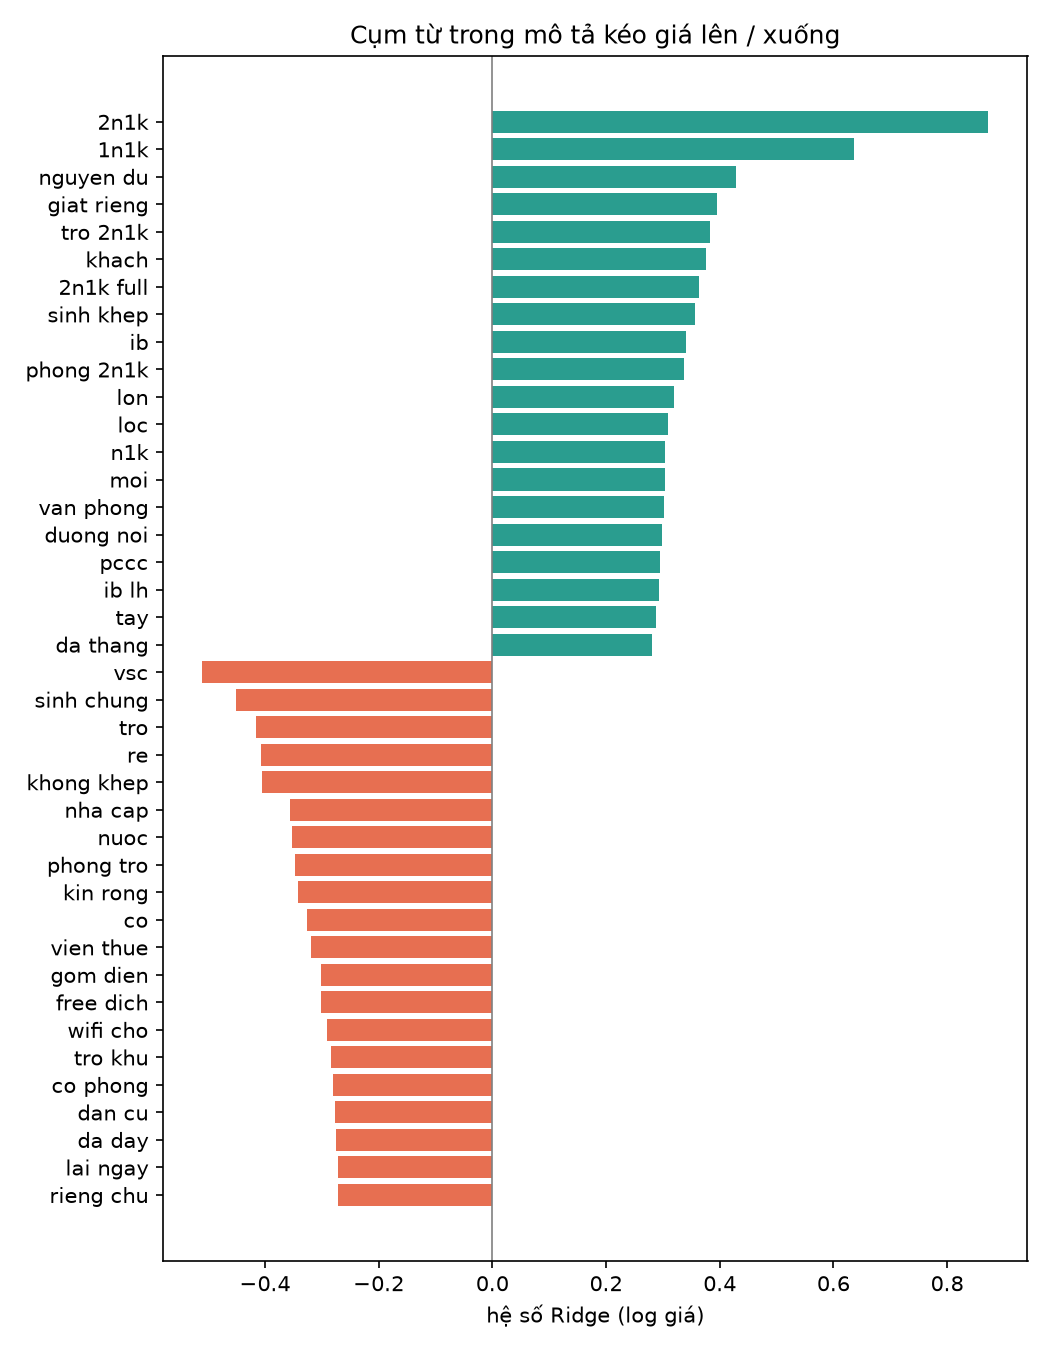
\includegraphics[width=\linewidth]{../../reports/figures/06_tfidf_coefficients.png}
  \caption{20 cụm từ trong mô tả có hệ số Ridge lớn nhất: kéo giá lên (xanh) và kéo giá xuống (cam).}
\end{minipage}\hfill
\begin{minipage}[t]{0.47\textwidth}
  \centering
  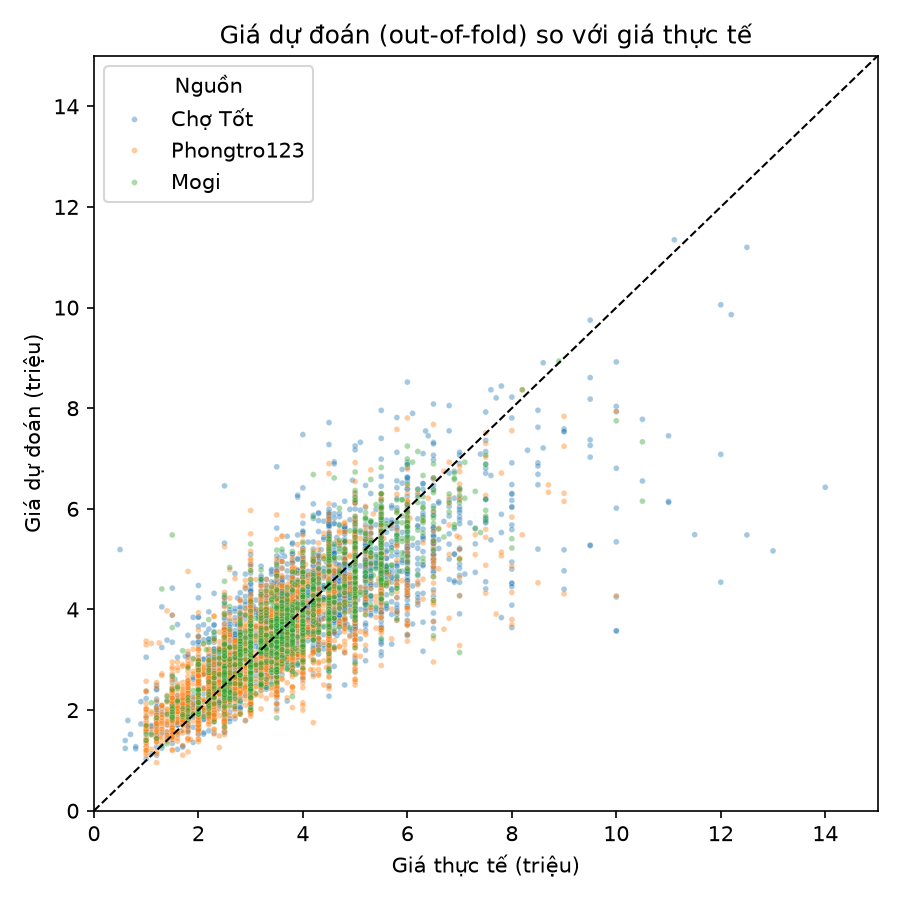
\includegraphics[width=\linewidth]{../../reports/figures/07_pred_vs_actual.png}
  \caption{Giá dự đoán out-of-fold (GroupKFold) so với giá thực tế; đường chéo là dự đoán đúng.}
\end{minipage}

\vspace{12pt}
\begin{minipage}[t]{0.47\textwidth}
  \centering
  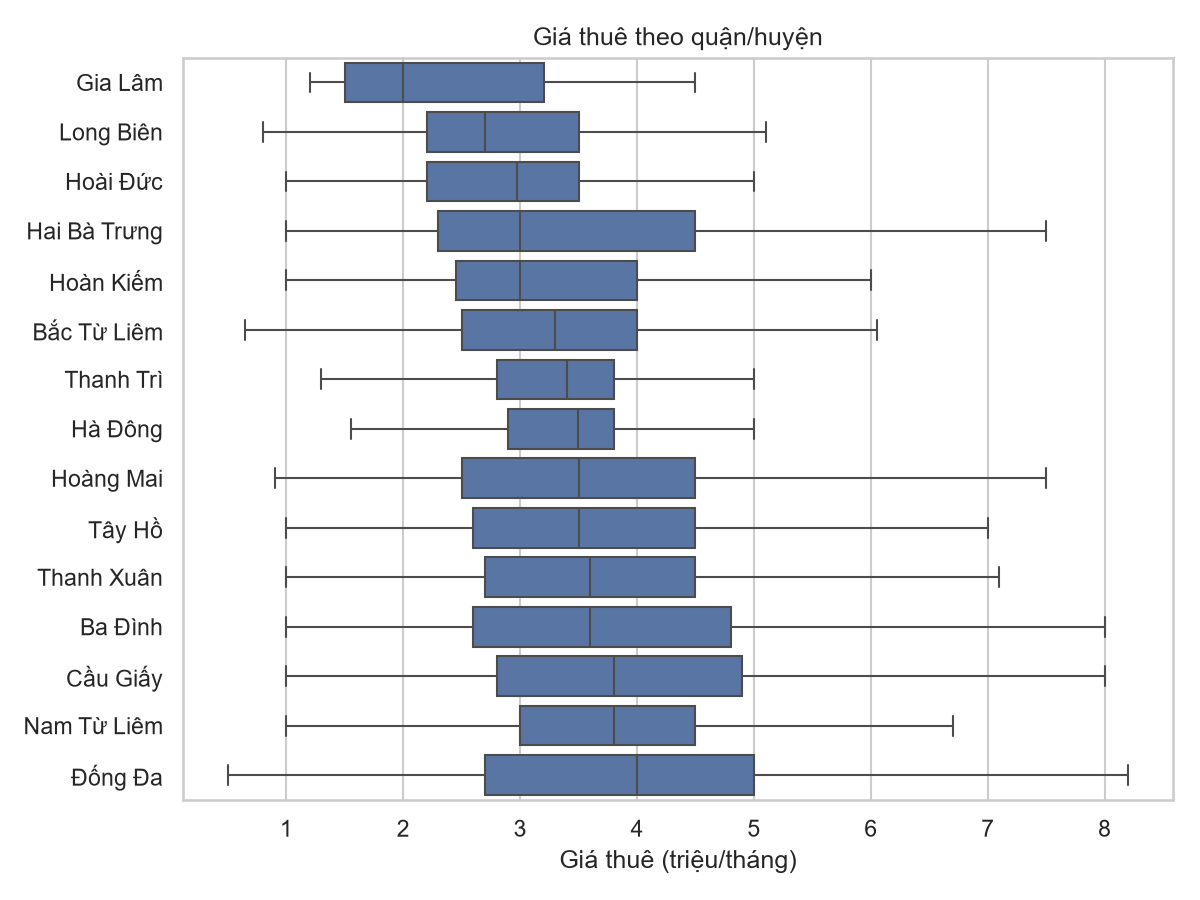
\includegraphics[width=\linewidth]{../../reports/figures/02_price_by_district.png}
  \caption{Giá thuê theo quận (các quận có ít nhất 30 tin, sắp theo giá trung vị).}
\end{minipage}\hfill
\begin{minipage}[t]{0.47\textwidth}
  \centering
  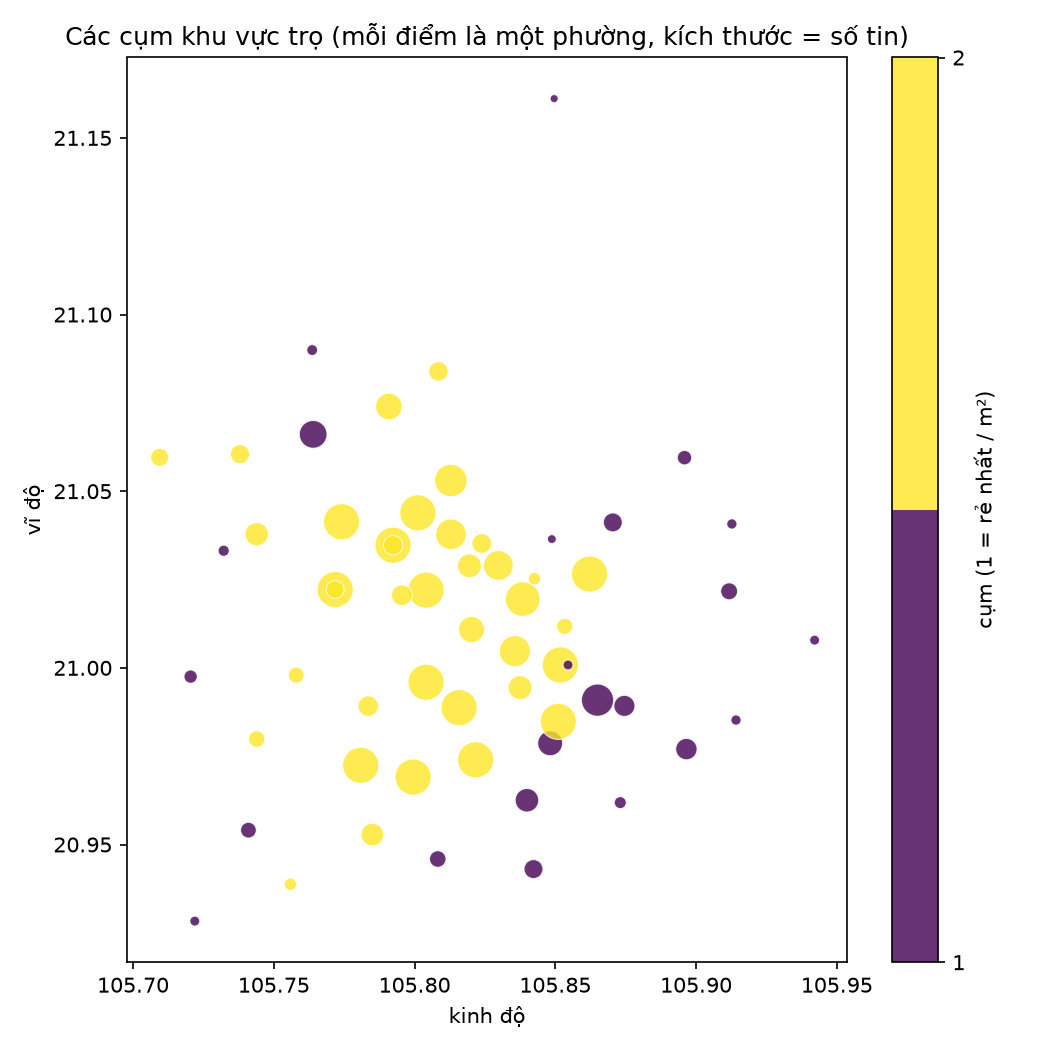
\includegraphics[width=\linewidth]{../../reports/figures/09_cluster_map.png}
  \caption{Phân cụm K-Means 60 phường: khu giá thấp và khu giá cao; kích thước điểm theo số tin.}
\end{minipage}
\end{figure}

\end{document}
